\documentclass{cup-ino}
\usepackage[utf8]{inputenc}
\usepackage{longtable}
\usepackage{blindtext,alltt}
%% Full title
\title{Weekly meeting notes}

%% Shorter title, for use in page header
\runningtitle{Template for CUP-INO}
\author{Eugenio Pescimoro, Marco Dentz, Juan J. Hidalgo}

%% The .bib file containing reference entires, for use with biblatex. CUP-INO loads the biblatex-chicago package with customisations for INO.
\addbibresource{refs.bib}

\begin{document}

\maketitle

\begin{abstract}
The aim of these notes is to describe one of the available numerical methods for modelling the diffusion and reaction processes of liquid chemical compounds displacing through fractured porous media.
\end{abstract}

\begin{figure}[bt!]
\begin{minipage}{0.47\textwidth}
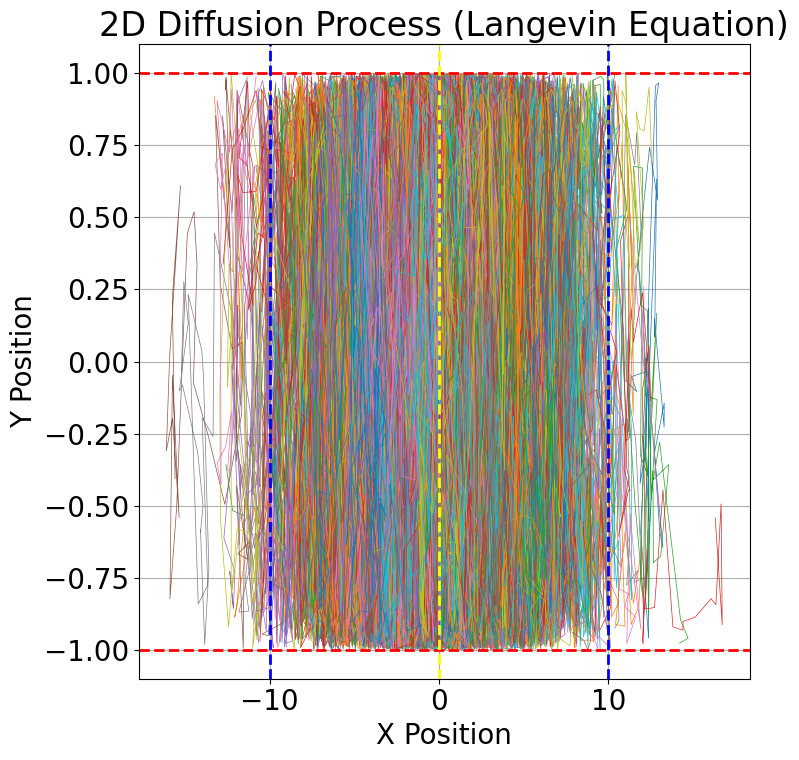
\includegraphics[width=\linewidth]{images/trajectoriesInfinite.png}
\floatnotes[]{Trajectories of 1e4 particles during 1e3 time steps}
\end{minipage}
\hfill
\begin{minipage}{0.47\textwidth}
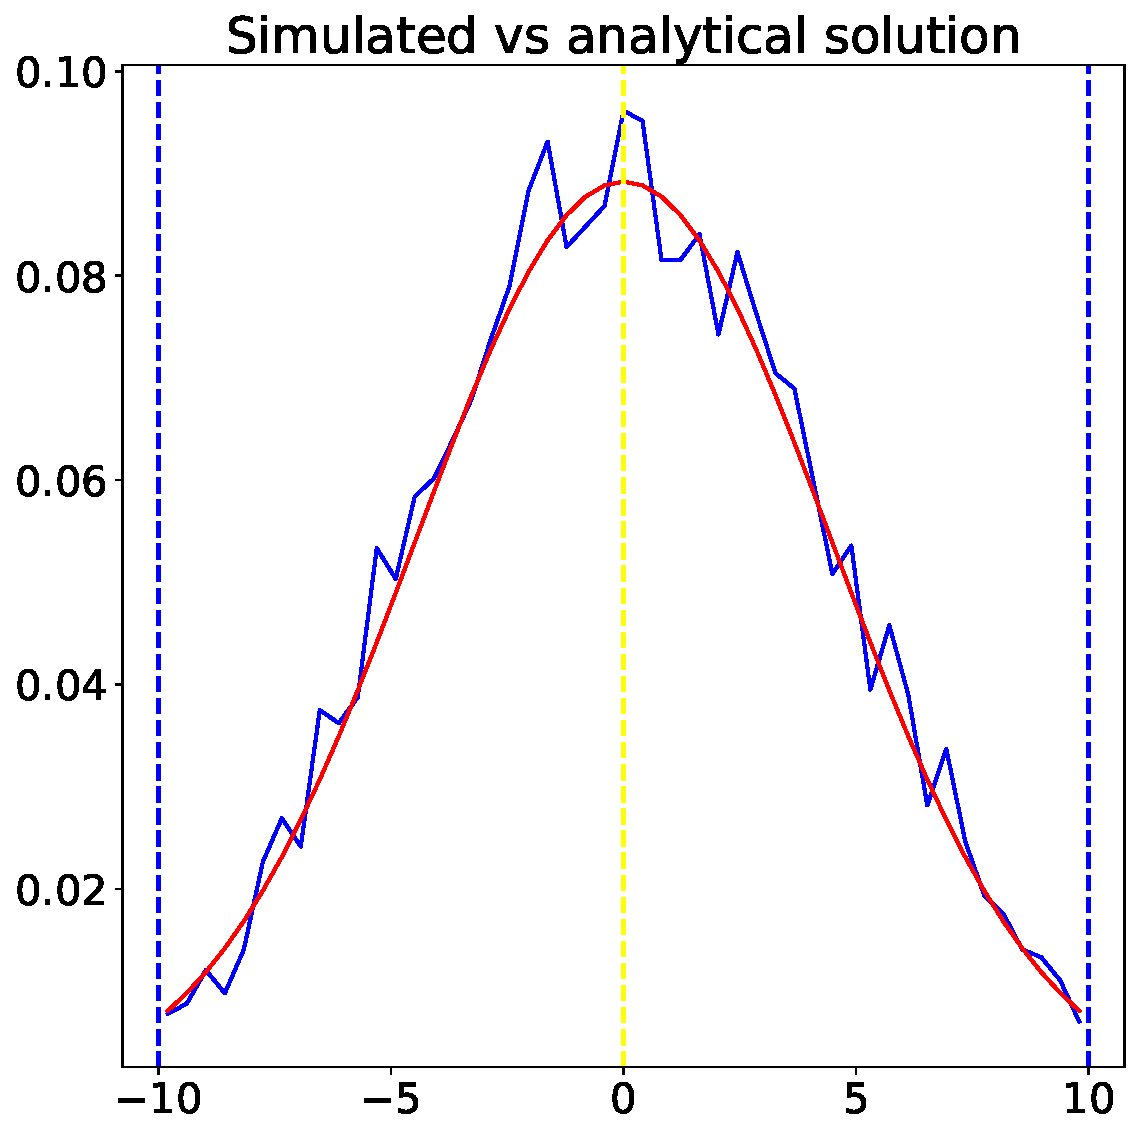
\includegraphics[width=\linewidth]{images/verificationInfinite.pdf}
\floatnotes[]{Spatial distribution of the particles at time 1e2}
\end{minipage}
\caption{Verification of the code comparing two spatial distribution of the concentration at a given time: solid blue line represents the spatial concentration from a numerical simulation while solid red line shows the analytical solution of the spatial concentration in a infinite domain at the same given time}
\label{fig:twosubs}
\end{figure}

\begin{figure}[bt!]
\begin{minipage}{0.47\textwidth}
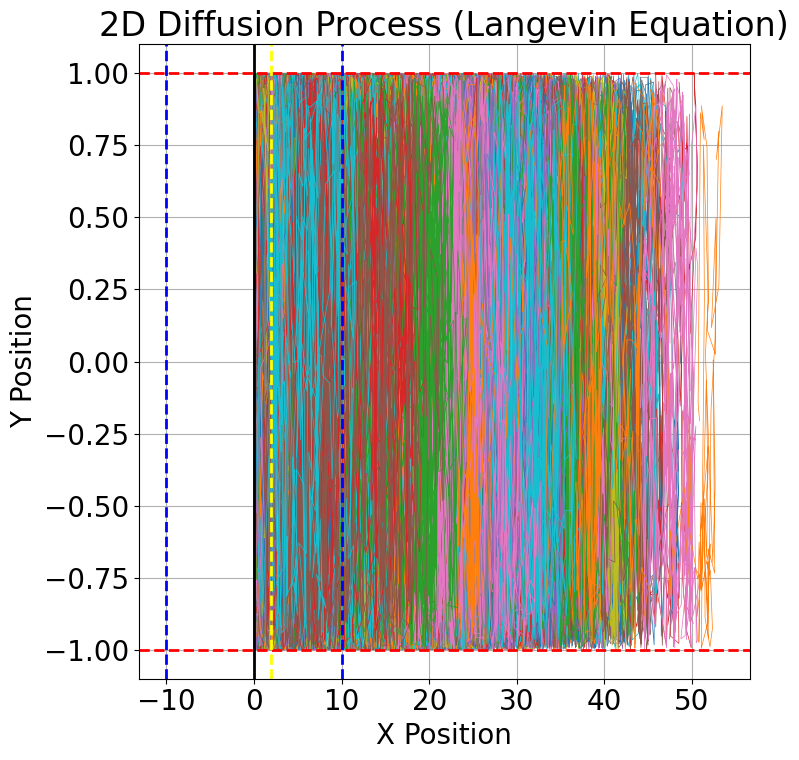
\includegraphics[width=\linewidth]{images/trajectoriesSemiInfinite.png}
\floatnotes[]{Trajectories of 1e4 particles during 1e3 time steps}
\end{minipage}
\hfill
\begin{minipage}{0.47\textwidth}
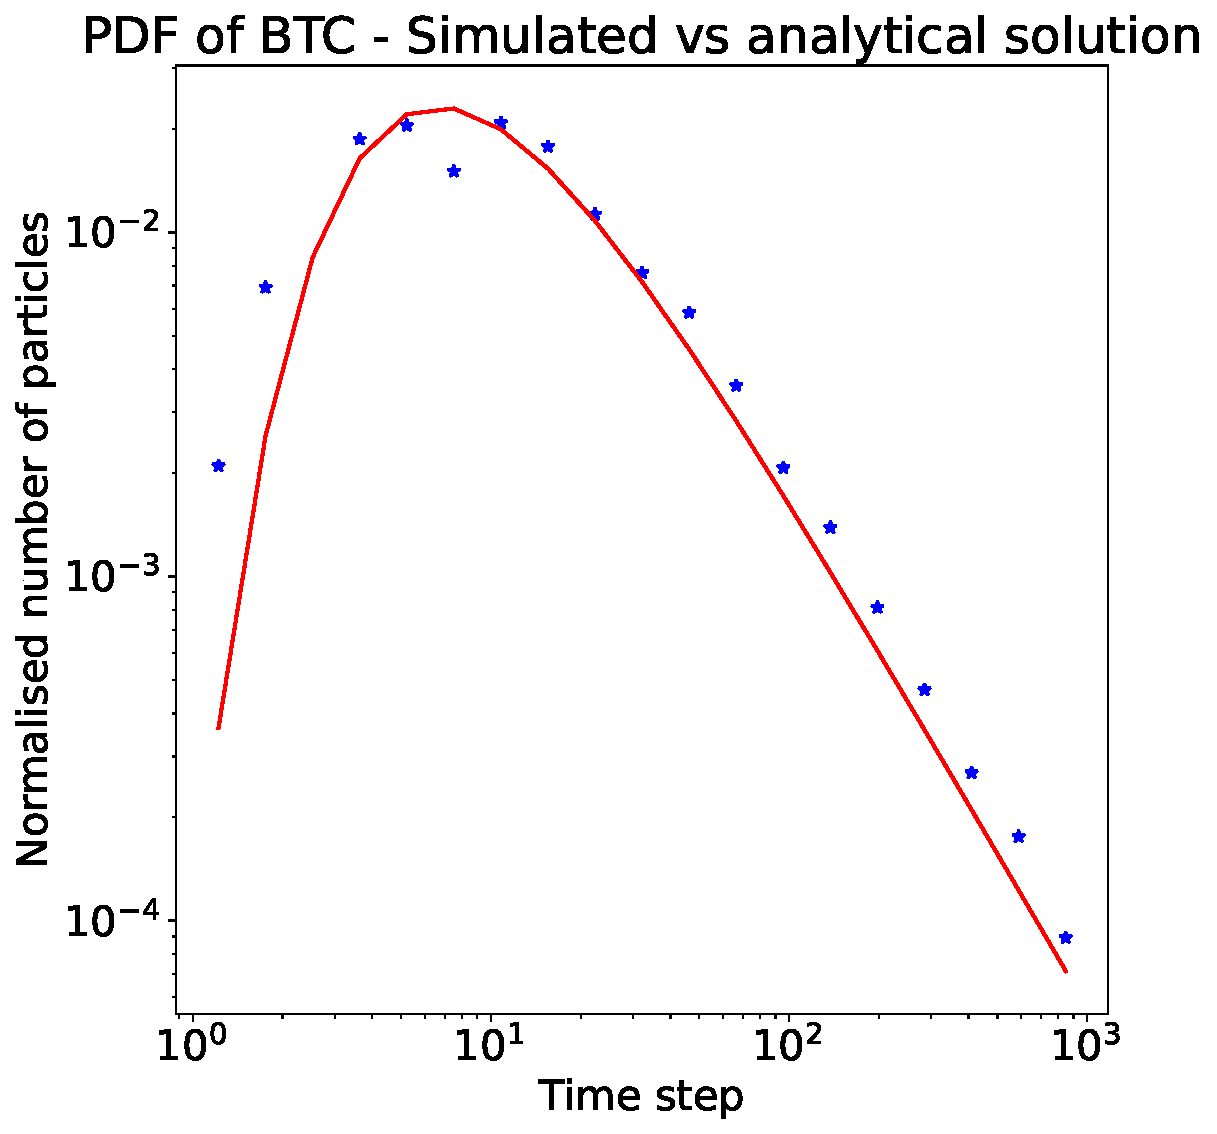
\includegraphics[width=\linewidth]{images/verificationSemi-infinite.pdf}
\floatnotes[]{Arrival times on the left absorbing boundary}
\end{minipage}
\caption{Verification of the code comparing two pdfs of the btc: blue dots represent the btc pdf from numerical simulation, solid red line is the analytical solution of the btc pdf for a semi-infinite domain}
\label{fig:twosubs}
\end{figure}

\noindent Here's an example citation\footcite{ries:sweeney} using the \verb|\footcite{...}| command from the \texttt{biblatex} package. There isn't a good, up-to-date BibTeX style for the Chicago style, so we're using the \texttt{biblatex} style \texttt{biblatex-chicago} instead. This means you'll need to run \texttt{biber} instead of \texttt{bibtex} if you're compiling this template on your local \LaTeX{} installation: on Overleaf, \texttt{biber} is run automatically. Note also that INO uses the Chicago author-year referencing style, but uses footnote citations. You can add pre-notes\footcite[See also][]{risse:2000} and post-notes\footcite[52]{checkel:1997}\footcite[119]{grieco:1993} with citations\footcite{simmons:2001} too, as well as multiple citations\footcite{elliot:1994,kilroy:1995,pauwelyn:2015,mastanduno:1996} in a single \verb|\footcite{...}|. Sometimes you may need to use\footnote{For an alternate treatment see \cite{ussenate:chemwarfare:1984} instead.} \verb|\cite{...}| in a \verb|\footnote{...}| as well. 

For a source with more than three authors,\footcite{inman:etal:2013} the note should include only the first author's name and et al. When more than one work by the same author is cited, that author's name is written out for each bibliographic entry, not replaced with ---.

No entry in the reference list is needed for newspaper or magazine articles; instead, include relevant information in a footnote.\footnote{\emph{Los Angeles Times}, 3 May 1993, A1} Article titles and authors are omitted except when including them would enhance understanding of points made in the text or the source.

Similarly, no entry in the reference list is needed for unpublished interviews. Instead, include relevant information in a footnote.\footnote{Author's interview with James Murphy, Washington, DC, July 1990} If the interviewee was promised anonymity, describe Guidelines for Contributors 253 the informant as precisely as possible---for example, as a member of a category of individuals---without identifying the person.

\paragraph{Author Anonymization}
Omit self-references that reveal your identity. You can modestly cite your own work without using pronouns that reveal your identity. Do not use references to ``Author'' when these are likely to reveal your identity. If needed, you can use the \texttt{censor} package\footnote{\url{https://ctan.org/pkg/censor}} to redact portions of text that may identify the authors.

\section{Example of a first section}

Figure \ref{fig:example} shows a normal figure, while figure \ref{fig:twosubs} show one made up of two sub-figures. Figure \ref{fig:landscape} is an example of a landscaped figure. You can use\footcite{simmons:2014} the \verb|\floatnotes{...}| command to add notes below figures\footcite{halimi:1990}.

\begin{table}
\caption{Automobile Land Speed Records (GR 5-10).}\label{tab:example}

\begin{tabular}{@{} l l l l r @{}}
\toprule
% \headrow
\emph{Speed (mph)} & \emph{Driver} & \emph{Car} & \emph{Engine} & \emph{Date}     \\
\midrule[\heavyrulewidth] %% Required by INO
407.447     & Craig Breedlove & Spirit of America          & GE J47    & 8/5/63   \\
413.199     & Tom Green       & Wingfoot Express           & WE J46    & 10/2/64  \\
434.22      & Art Arfons      & Green Monster              & GE J79    & 10/5/64  \\
468.719     & Craig Breedlove & Spirit of America          & GE J79    & 10/13/64 \\
526.277     & Craig Breedlove & Spirit of America          & GE J79    & 10/15/65 \\
536.712     & Art Arfons      & Green Monster              & GE J79    & 10/27/65 \\
555.127     & Craig Breedlove & Spirit of America, Sonic 1 & GE J79    & 11/2/65  \\
576.553     & Art Arfons      & Green Monster              & GE J79    & 11/7/65  \\
600.601     & Craig Breedlove & Spirit of America, Sonic 1 & GE J79    & 11/15/65 \\
622.407     & Gary Gabelich   & Blue Flame                 & Rocket    & 10/23/70 \\
633.468     & Richard Noble   & Thrust 2                   & RR RG 146 & 10/4/83  \\
763.035     & Andy Green      & Thrust SSC                 & RR Spey   & 10/15/97\\
\bottomrule
\end{tabular}

\floatnotes{Data from \url{https://www.sedl.org/afterschool/toolkits/science/pdf/ast_sci_data_tables_sample.pdf}}

\end{table}

Lorem ipsum dolor sit amet, consectetur adipiscing elit, sed do eiusmod tempor incididunt ut labore et dolore magna aliqua. Ut enim ad minim veniam, quis nostrud exercitation ullamco laboris nisi ut aliquip ex ea commodo consequat. Duis aute irure dolor in reprehenderit in voluptate velit esse cillum dolore eu fugiat nulla pariatur. Excepteur sint occaecat cupidatat non proident, sunt in culpa qui officia deserunt mollit anim id est laborum.

Lorem ipsum dolor sit amet, consectetur adipiscing elit, sed do eiusmod tempor\footnote{Example of a normal footnote} incididunt ut labore et dolore magna aliqua. Ut enim ad minim veniam, quis nostrud exercitation ullamco laboris nisi ut aliquip ex ea commodo consequat. Duis aute irure dolor in reprehenderit in voluptate velit esse cillum dolore eu fugiat nulla pariatur. Excepteur sint occaecat cupidatat non proident, sunt in culpa qui officia deserunt mollit anim id est laborum.

Lorem ipsum dolor sit amet, consectetur adipiscing elit, sed do eiusmod tempor inciddt enim ad minim veniam, quis nostrud exercitation ullamco laboris nisi ut aliquip ex ea commodo consequat. 


\begin{figure}
\centering
\includegraphics[width=0.8\textwidth]{example-image}
\floatnotes{Here are some notes. Here are some notes. Here are some notes. Here are some notes. Here are some notes. Here are some notes. Here are some notes. Here are some notes. Here are some notes. Here are some notes.}
\caption{This is a figure caption}
\label{fig:example}
\end{figure}


\begin{figure}[bt!]
\begin{minipage}{0.47\textwidth}
\includegraphics[width=\linewidth]{example-image}
\floatnotes[]{A brief note for a subfigure.\\\emph{Source:} the source}
\end{minipage}
\hfill
\begin{minipage}{0.47\textwidth}
\includegraphics[width=\linewidth]{example-image}
\floatnotes[]{A brief note for a subfigure.\\\emph{Source:} the source}
\end{minipage}

\caption{This is a caption for the entire figure}
\label{fig:twosubs}
\end{figure}

\begin{sidewaysfigure}
\centering
\includegraphics[width=14cm]{example-image}
\floatnotes{Here are some notes. Here are some notes. Here are some notes. Here are some notes. Here are some notes. Here are some notes. Here are some notes. Here are some notes. Here are some notes. Here are some notes.}
\caption{This is a figure caption}
\label{fig:landscape}
\end{sidewaysfigure}

\blinddocument

A supplementary material section will always appear before the (optional) Appendix and Reference list. If you're certain that your submission won't have any supplementary material, you can add the \texttt{nosupp} option to the document class declaration, i.e. 
\begin{quote}
\verb|\documentclass[nosupp]{cup-ino}|    
\end{quote}

%% Optional appendix
\appendix

\begin{figure}[hbt!]
    \centering
    \includegraphics[width=4cm]{example-image}
    \caption{Appendix figure}
    \label{app:fig}
\end{figure}

\begin{table}[hbt!]
    \caption{Appendix table}
    \label{app:tab1}
\begin{tabular}{c c c c c}
\toprule
     abc & def & ghi & jkl & mno \\
\midrule
     abc & def & ghi & jkl & mno \\
     abc & def & ghi & jkl & mno \\
     abc & def & ghi & jkl & mno \\
     abc & def & ghi & jkl & mno \\
     abc & def & ghi & jkl & mno \\
\bottomrule
\end{tabular}
\end{table}


\printbibliography

\section*{Authors}
\begin{authorbio}
\textbf{Author One} is lorem ipsum dolor sit amet, consectetur adipiscing elit, sed do eiusmod tempor incididunt ut labore et dolore magna aliqua. She can be reached at abc@xyz.edu.

\textbf{Author Two} is \ldots. He can be reached at foo@bar.edu.
\end{authorbio}

\section*{Acknowledgements}
We thank\ldots

\section*{Key Words}
Keyword one; keyword two; keyword three; keyword four.

\end{document}
